\section{StyleGAN + CycleGAN}
\begin{frame}
    \frame{\frametitle{Module 23.1: Generative Adversarial Networks - StyleGAN + CycleGAN}}

	% \myheading{Section 5: StyleGANs}
\end{frame}

\begin{frame}
    \begin{figure}[h!]
        \hyperlink{StyleGAN}{
        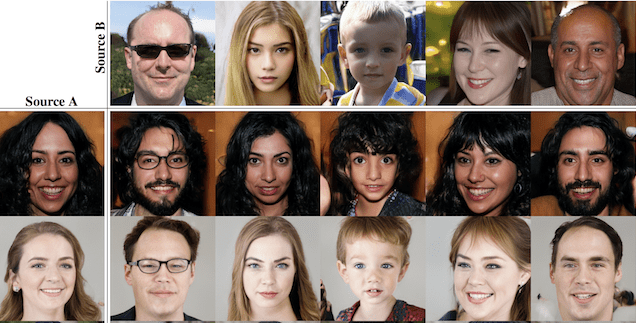
\includegraphics[scale=0.40]{images/stylegan_example1.png}
        \caption{Example of One Set of Generated Faces (Left) Adopting the Coarse Style of Another Set of Generated Faces (Top) Taken from: A Style-Based Generator Architecture for Generative Adversarial Networks.}
        }
	\end{figure}
	\begin{itemize}
		\item<1-> GAN: Lacking Control Over Synthesized Images
		\item<2-> Style Generative Adversarial Network(StyleGAN) Controls Style Using New Generator Model
        \item<3-> StyleGan is proficient in producing impressively photorealistic high-quality photos of faces and grants control over the characteristic of the created image at different specification levels by changing the style vectors and noise.
	\end{itemize}
        
\end{frame}

\begin{frame}
    \frametitle{StyleGAN Model Architecture}
    \hyperlink{StyleGAN}{
    	\begin{figure}[h!]
    		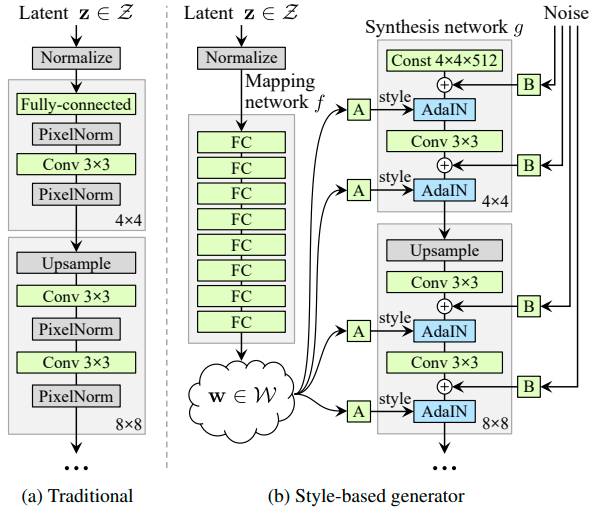
\includegraphics[scale=0.40]{images/StyleGan_Architecture.png}
    	\end{figure}
     }
    \textbf{The StyleGAN is described as a progressive growing GAN architecture with five modifications, each of which was added and evaluated incrementally in an ablative study.
    The incremental list of changes to the generator are:}
    \begin{itemize}
        \item Baseline Progressive GAN.
        \item Addition of tuning and bilinear upsampling.
        \item Addition of mapping network and AdaIN (styles).
        \item Removal of latent vector input to generator.
        \item Addition of noise to each block.
        \item Addition Mixing regularization.
    \end{itemize}

\end{frame}

\begin{frame}
    \frametitle{CycleGAN}
    \textbf{Style transfer problem: change the style of an image while preserving the content.}
    \hyperlink{CycleGAN}{
    	\begin{figure}[h!]
    		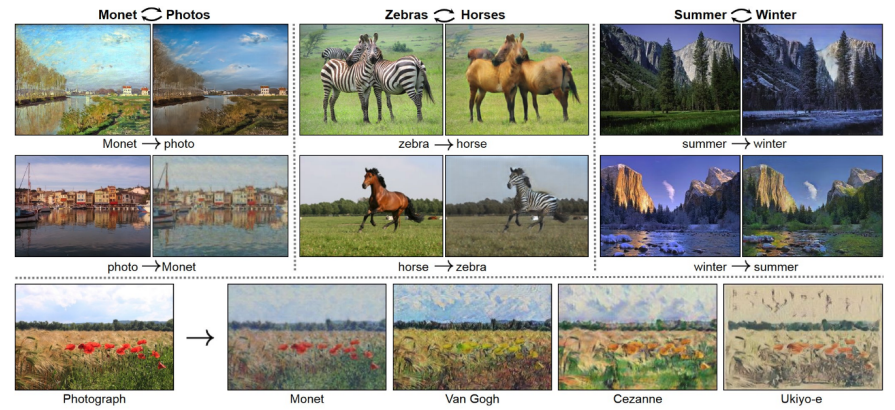
\includegraphics[scale=0.40]{images/cyclegan1.png}
    	\end{figure}
     }
    \textbf{Data: Two unrelated collections of images, one for each style}
\end{frame}

\begin{frame}
    \title{CycleGAN}
    \begin{itemize}
        \item If we had paired data (same content in both styles), this would be a supervised learning problem. But this is hard to find.
        \item The CycleGAN architecture learns to do it from unpaired data.
        \begin{itemize}
            \item Train two different generator nets to go from style 1 to style 2, and vice versa.
            \item Make sure the generated samples of style 2 are indistinguishable from real images by a discriminator net.
            \item Make sure the generators are cycle-consistent: mapping from style 1 to style 2 and back again should give you almost the original image.
        \end{itemize}
    \end{itemize}
\end{frame}

\begin{frame}
    \title{CycleGAN}
    \hyperlink{CycleGAN}{
    	\begin{figure}[h!]
    		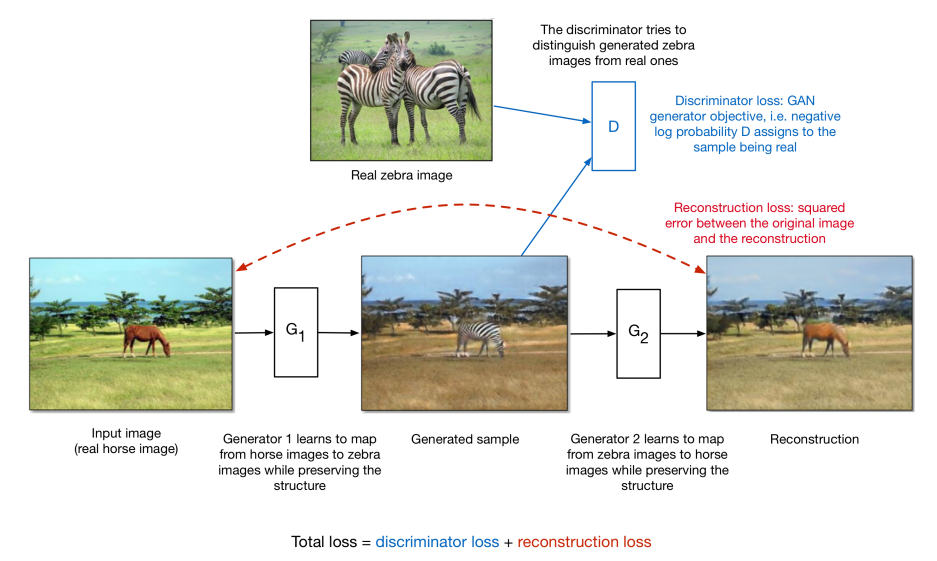
\includegraphics[scale=0.40]{images/cyclegan2.png}
    	\end{figure}
     }
\end{frame}

\begin{frame}
    \title{CycleGAN}
    \textbf{Style transfer between aerial photos and maps:}
    \hyperlink{CycleGAN}{
    	\begin{figure}[h!]
    		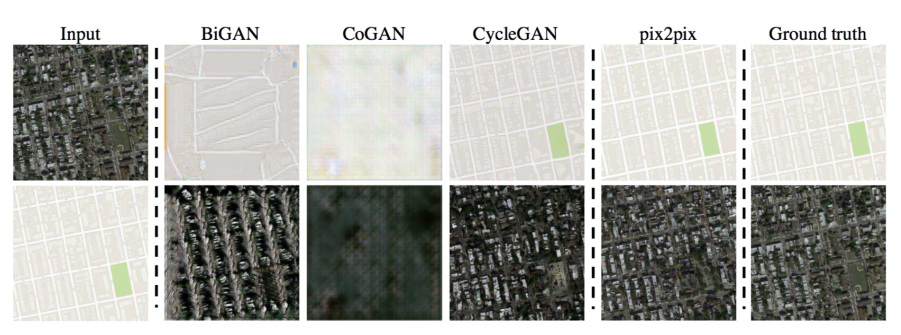
\includegraphics[scale=0.40]{images/cyclegan3.png}
    	\end{figure}
    }
\end{frame}

\begin{frame}
    \title{CycleGAN}
    \textbf{Style transfer between road scenes and semantic segmentations (labels of every pixel in an image by object category):}
    \hyperlink{CycleGAN}{
    	\begin{figure}[h!]
    		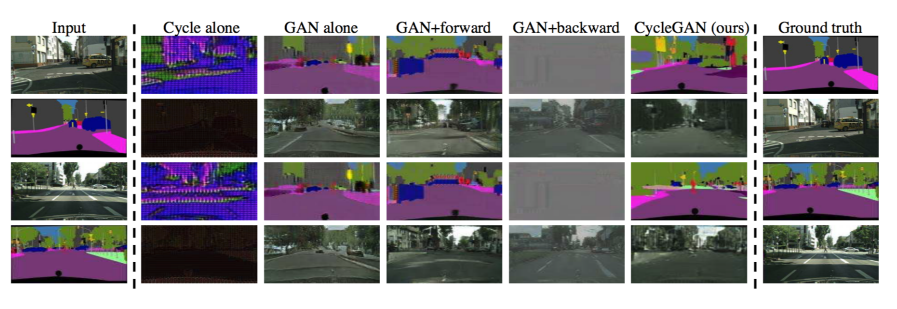
\includegraphics[scale=0.40]{images/cyclegan4.png}
    	\end{figure}
    }
\end{frame}
